\chapter{The Health Effects of Early Interventions}

\fancyhead[L]{ECON0024}
\fancyhead[C]{Ch.4 The Health Effects of Early Interventions}
\fancyhead[R]{Kaicheng Lu}
\fancyfoot[L]{\hyperlink{tableofcontents}{Back to Table of Contents}}
\fancyfoot[R]{Kaicheng Lu}
 
\section{Questions we are interested in and motivation}

    \begin{itemize}
        \item We saw the substiantial SES-health gradient last time
        \item Moreover, \href{https://www.sciencedirect.com/science/article/pii/S0047272720300359}{Attanasio, Blundell. Conti and Mason (2019)} showed that this inequality is multidimentional. Inequality in socio-emotional skills (mental health) of 5 year olds has also widened over time.
        \begin{itemize}
            \item  The score on various socio-emotional skills were normalised to 0 for the 1970 cohort, and we can see from figure \ref{SMinequality} that kids born to more educated mothers are better off in 2000 compared to 1970 (gap became bigger).
            \item Interpreting the fig: externalising = social skills; internalising = the ability to focus; higher value is better
        \end{itemize}
        \begin{figure}[H]%option [H] means "strictly here"
            \centering
            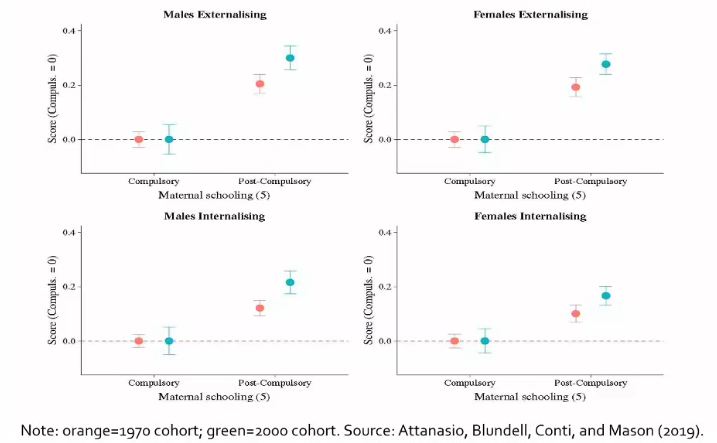
\includegraphics[width=13cm]{images/ch4/socioemotional inequality.png}
            \caption{inequality in socio-emotional skills}
            \label{SMinequality}
        \end{figure}
        \item What should we do?
        \begin{itemize}
            \item Try to look at the forgotten aspect in the Grossman health production model: early childhood development
            \item From the data, about a half of the difference in labour market outcomes, health behaviour and health at age 30 can be explained by early life factors happening before $\leq$ 10 years old, and the rest is explained by the causal effect of edu \href{https://www.nber.org/system/files/working_papers/w18466/w18466.pdf}{(Conti and Heckman, 2010)}
            \item Traits of health inequality also begin early in life: high value of C-Reactive Protein (a measure of inflammation) was documented at mid-40s for those in low SES. At the same time, a similar gradient occurred in childhood, where children born to lower SES households are also more likely to have low birth weight \href{https://www.nber.org/system/files/working_papers/w18466/w18466.pdf}{(Conti and Heckman, 2010)}
             \item SES-health gradient can occur before birth! The fact that the mother resides in deprived neighbourhoods had a significant negative effect on the size of fetus along different dimensions \href{https://www.econstor.eu/bitstream/10419/200319/1/1047143135.pdf}{(Conti et al., 2018)} 
            \begin{figure}[H]%option [H] means "strictly here"
                \centering
                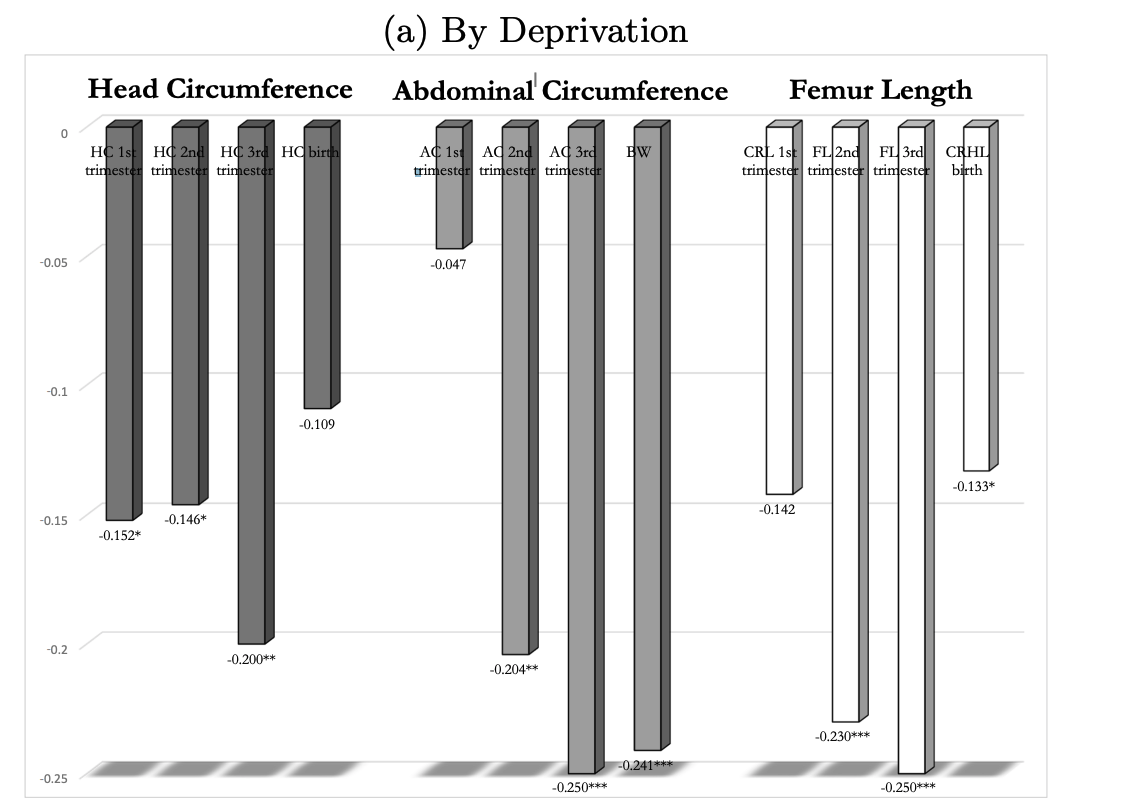
\includegraphics[width=13cm]{images/ch4/Prebirth gradient.png}
                \caption{SES-health gradient before birth}
                \label{Prebirthgradient}
            \end{figure}
            \item This means that the fetuses of poorer moms are smaller, so you will have smaller babies as gestation continues.
            \item The key takeaway from all these stories is that when the kid is conceived, there are already inequalities that will be carried over throught the lifecycle
        \end{itemize}
    \end{itemize}
    
    \textbf{OK maybe it makes sense to start early!} 


\section{Understanding the causal effect of early life conditions}

    \begin{itemize}
        \item The way to look for causal effects involves techniques in labor (quasi-natural experiments from exposure to war, pandemics, policies) and twin-based designs (twin FE, how does the outcome of the high-birth-weight twin look like?)
        \item Here, we look at effect of early childhood conditions on later life outcomes by  exploiting policy shocks and RCTs
        \item A slight detour before studying effect of various internventions: some major findings in the literature on this topic:
        \begin{itemize}
            \item The effect of early shocks are heterogeneous, and the heterogeneity is endogenous. Effect of shocks depends on child endowments, resource constraints and production technologies
            \item Limited understanding on effect of multiple shocks, and the relative importance of biology and behavioural mechanisms
        \end{itemize}
        \item Nevertheless, we should intervene becuase there are frictions preventing parental investment in human capital in early years, such as...
        \begin{itemize}
            \item Information and liquidity constraint
            \item Behavioral factors: Time inconsistency, altruism, cognitive constraints, aspirations
        \end{itemize}
        \item Interventions may help: fetus of smoking moms' are much smaller. A slight caveat here is that higher obesity in the population can lead to too big fetuses (bigger $\neq$ better).
    \end{itemize}


\section{We should intervene. But intervene how?}

    \subsection{Pre-natal Interventions: Home visiting (HV)}
    
        \subsubsection{Nurse Family Partnerships (NFP)}
        
            \begin{itemize}
                \item A program very popular in the USA
                \item Nurses going to houses of first-time low-SES mothers at early stage of pregnancy until the child is 2 years old
                \item Max. 64 visits that provide information and support
                \item Super high return ($\approx$ 500\%)
                \item Treated kids (those with parents being allocated to NFP group) turned out better in terms of better cognition, higher likelihood to graduate high school with honours, less disabilities, and the mothers spent less money in welfare compared to the control group (those with parents allocated to not-that-good usual care system)
                \item Details on cost-saving (\href{https://publications.aap.org/pediatrics/article/144/6/e20183889/77004/Prenatal-and-Infancy-Nurse-Home-Visiting-Effects}{Olds et al., 2019}):
                \begin{figure}[H]%option [H] means "strictly here"
                    \centering
                    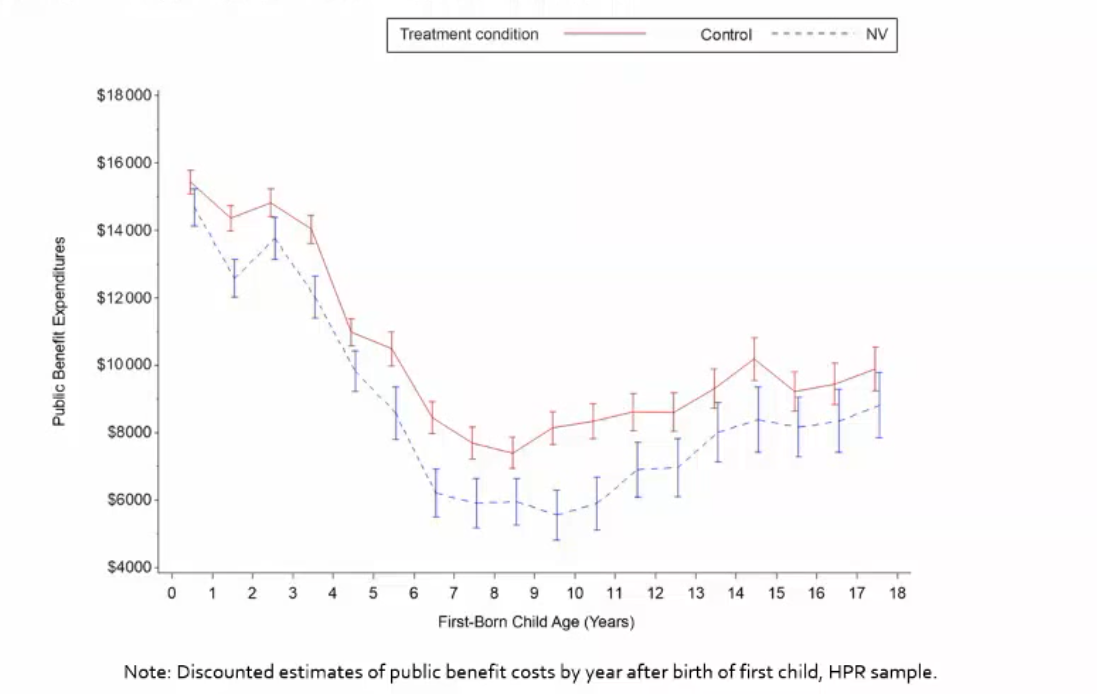
\includegraphics[width=13cm]{images/ch4/NFP cost saving.png}
                    \caption{Cost saving in NFP (NV) group}
                    \label{Prebirthgradient}
                \end{figure}
                \textbf{So NFP effective and saves money for the government? We cannot say that until we consider what will happen if we scale this up!}
            \end{itemize}
            
        \subsubsection {Scaling up}
        
            \begin{itemize}
                \item This is a relatively new area of research, and we have relatively good evidence on the effect of HV at scale from Scandinavian countries due to their ``welfare state" setup
                \item \href{https://www.aeaweb.org/articles?id=10.1257/app.20150087}{Hjort et al. (2017)} studied a HV program that was implemented at scale in Denmark from 1937-49
                \item They found that kids in treated areas saw huge improvements in SES and health compared to the control group (note that this effect is for every child in Denmark!)
                \item Some examples of improvement:
                \begin{itemize}
                    \item Children in treated areas more likely to survive after 64 years old
                    \item Less likely to be diagnosed with diseases
                    \item Fewer nights spent in hospitals
                \end{itemize}
            \end{itemize}
            
        \subsubsection{That's Great! But the effect of HV in the UK is unknown due to data problems...}
        
            We also have similar programs in the UK called the Healthy Child Programme (HCP) that ...
            \begin{itemize}
                \item provided advice \& support (e.g.immunization, examination of the child)
                \item Identified risks (e.g. abuse)
                \item Referral to social services if needed
            \end{itemize}
            \textbf{Is it effective? We don't know because there is no data!}
            \\ \\
            However, this program is now facing its own problems
            \begin{itemize}
                \item Massive defunding after Oct 2015 \& local authorities taking over this responsibility
                led to caseload of $>$500 in some regions
                \item Health visitors were moved to the frontline during 
                \item The effect of this is by no means trivial. A survey of visitors by \href{https://discovery.ucl.ac.uk/id/eprint/10106430/8/Conti_Dow_The%20impacts%20of%20COVID-19%20on%20Health%20Visiting%20in%20England%20250920.pdf}{Conti and Dow (2020)} showed that they are concerned about domestic abuse \& violence, parents' mental health, child growth/ development, ...
            \end{itemize}

        \subsubsection{Does the success of the NFP generalise? Investigation of the Family Nurse Partnership (FNP) programme in the UK}
        
            \begin{itemize}
                \item Note the difference between the UK FNP and the US NFP :)
                \item Eligibility criteria of FNP: teenage first-time mom (regardless of SES)
                \item This program was scaled up after being implemented in small scale (10 sites) and received positive feedback
                \item Result of an RCT that came out in 2014 showed that this program did not impact the primary outcomes. However, it improved other outcomes such as child cognitive \& language development, but they were considered secondary. Primary outcomes are health-based, see figure \ref{FNPgoal} for details on the outcomes of interest.
                \begin{figure}[H]%option [H] means "strictly here"
                \centering
                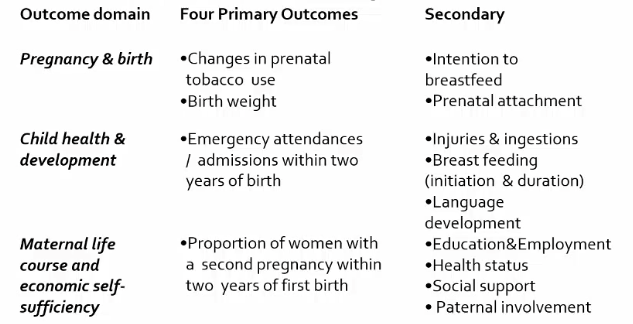
\includegraphics[width=10cm]{images/ch4/OutcomesInterest_FNP.png}
                \caption{Primary and Secondary outcomes in the UK FNP}
                \label{FNPgoal}
                \end{figure}
                \item Follow-up studies showed that the effect on cognitive development (reading and writing) persisted, but there was no impacts on child maltreatment
                \item \textbf{Overall, the program only improved certain aspects of child development, not others.} ``Adding FNP to the usually provided health and social care provided no additional short-term benefits to our primary outcomes"
            \end{itemize}
        
        \subsubsection{What could explain the poor generalizability of the evidence?}
            \begin{itemize}
                \item Difference in culture leading to different behaviour
                \item Difference in trust in public institutions
                \item Difference in counterfactual. The control group gets much worse treatment in the US compared to the UK (remember that control group in the UK gets HV!).
                \begin{itemize}
                    \item In FNP, households get about 39 visits. In control (HV), households get about 16 visits from NHS health visitors
                    \item FNP and HV can both tell mothers about how to make the kid healthy (breastfeeding, not smoking, ...). However, the unique thing about the FNP was that they told moms how to approach child cognitive development (e.g. play with the child)
                \end{itemize}
            \end{itemize}
            \textbf{Note that the secondary outcomes are still important, and the FNP does have a positive significant impact on child development at 5 \& 7 years old.}\\ \\
            \textbf{Also note that recent studies \href{https://jamanetwork.com/journals/jama/article-abstract/2793825?casa_token=hmQ4aJAMtL8AAAAA:22C4Pg2uXeayMj306ws_iqVE56LIoViTQfKUWIhJoXNQ4S9YLAZofvhEgmKVeFYWdOQ3800Tcj4}{(McConnell et al. 2022)} evaluating the effect of the US NFP found that it no longer brings significant improvements on `` maternal and newborn health primary or secondary outcomes". The effectiveness of programs can also change over time even for the same country due to different counterfactuals} 

    \subsection{Post-natal Interventions}
    
        \subsubsection{The Carolina Abecedarian Project}
            \begin{itemize}
                \item This is a small-scale randomised experiment in the US in the 1970s
                \item Send poor African-American kids to intensitve daycare from 0-5 years old
                \item What do they have at the daycare centres?
                \begin{itemize}
                    \item Cognitive and behavioural stimulations
                    \item Healthcare
                    \item Nutrition (food provision)
                \end{itemize}
            \item It is also very effective!
            \begin{itemize}
                \item Benefit-to-Cost Ratio = 7.3
                \item Group exposed to this treatment had better health in adulthood compared to the control
                    \begin{figure}[H]%option [H] means "strictly here"
                \centering
                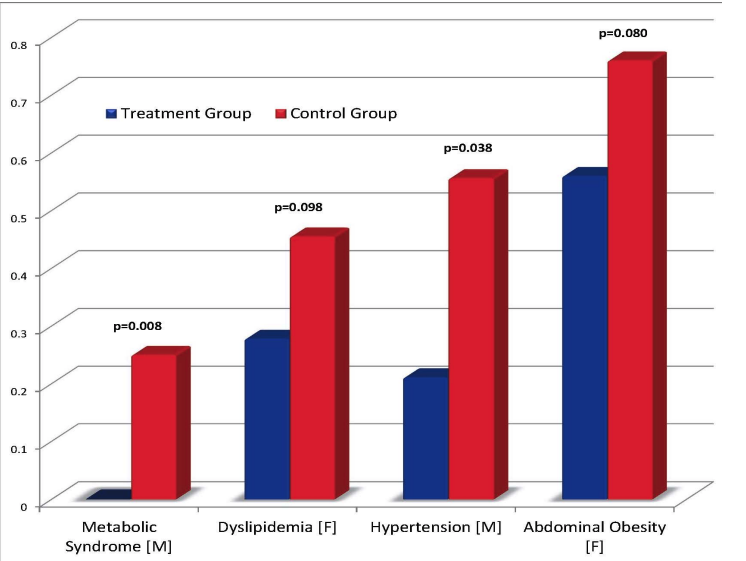
\includegraphics[width=8cm]{images/ch4/CAP_eval.png}
                \caption{Improved health in adulthood (35 yr old)}
                \label{CAP_eval}
                \end{figure}
            \end{itemize}
            \end{itemize}
            
        \subsubsection{Effect of implementing this at a larger scale: an examination of the effects of Head Start and Sure Start}
            \textbf{Head Start (US)}
            \begin{itemize}
                \item A compensatory preschool program in the US providing head start centres (centres providing a variety of services as in the CAP ) to low income children 
                \item \href{https://www.aeaweb.org/articles?id=10.1257/pol.6.4.135}{Carneiro and Ginja (2014)} found that ``participation in the program reduces the
            incidence of behavioural problems, health problems, and
            obesity of male children at ages 12 and 13; lowers depression
            and obesity among adolescents, and it reduces engagement in
            criminal activities and idleness for young adults."
                %shows that in spite of the lack of program impacts by first grade, there are important longer term impacts of Head Start on the health and criminal behavior of adolescents and young adults
                \item They employed a fuzzy RDD design using discontinuities
            in the probability of participation induced by program eligibility
            rules (note that a jump was only observed in males)
            \item Results in more detail: 
                    \begin{figure}[H]%option [H] means "strictly here"
                \centering
                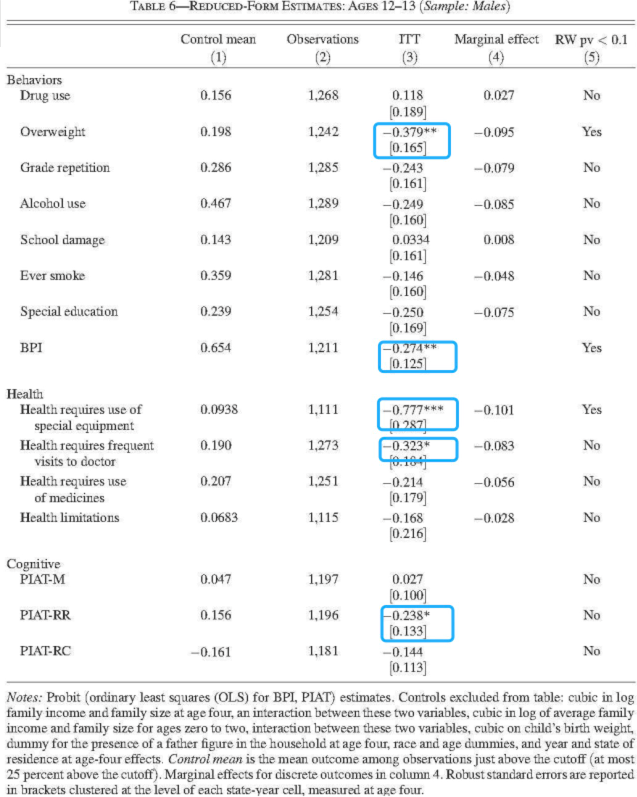
\includegraphics[width=11.5cm]{images/ch4/HSeval.png}
                \caption{Head Start reduces overweight, behavioural (BPI) and other problems for adolescents}
                \label{CAP_eval}
                \end{figure}
            \end{itemize}
            \textbf{Sure Start (UK)}
            \begin{itemize}
            \item This is a program launched in  1999 in England that was initially targeting diadvantaged communities but then scaled up
            \item The program intends to provide all the help possible to parents in one go
            \begin{itemize}
                \item Provision of health information 
                %via health visitors clinics and will refer to health services if needed
                \item Referral to health services
                \item Stay-and-play, parenting programmes (e.g. FNP)
                \item Parental support, job search assistance
            \end{itemize}
            \item The impact of this program is studied under the following framework:
            $$D^{ya}_{sql(d)}=\delta^{ya}SS_{dq}+\beta^{ya}X_s+\alpha^{ya}Pop_{al}+\gamma^{ya}_q+\pi^{ya}_{l(d)}+\epsilon^{ya}_{sql(d)} $$
            Where
            \begin{itemize}
            \item $D^{ya}_{sql(d)}$: an indicator for whether there is any hospitalization of type y at
        age $\alpha$ for children of sex s born in quarter q and residing in neighborhood l (of LA d)
        \item  $SS_{dq}$: the average number
        of centers per thousand children aged 0-4 that were open between the child’s birth and the age at
        which the outcome is measured
        \item Gender, size of population in the LAs are controlled for
        \item Also included chort of birth \& neighbourhood FEs
        \end{itemize}
        \item Results
        \begin{itemize}
            \item Sure Start reduces overall hospitalisations. Note that there was an increase in hospitalisation at the age of 1, and this is probably due to hospitalisation for preventative purposes
            \begin{figure}[H]%option [H] means "strictly here"
                \centering
                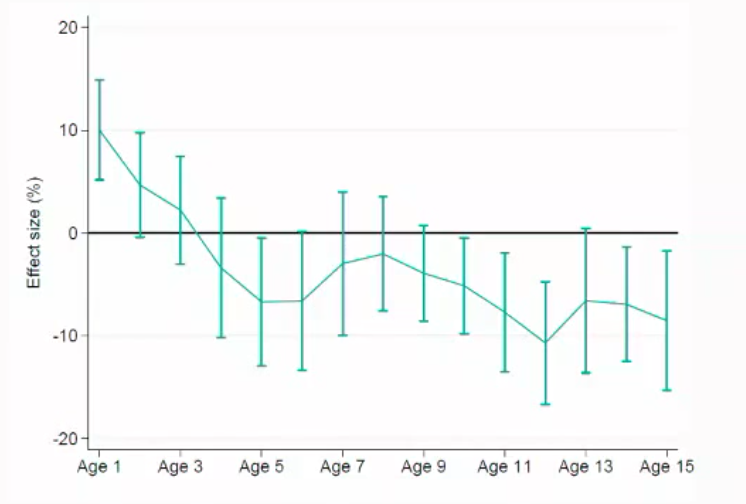
\includegraphics[width=7cm]{images/ch4/SS_overall.png}
                \caption{Sure Start reducing overall hospitalisation}
            \end{figure}
        \end{itemize}
        \item If we decompose by causes of hospitalisation and the extent to which treated areas are deprived
        \begin{figure}[H]%option [H] means "strictly here"
            \centering
            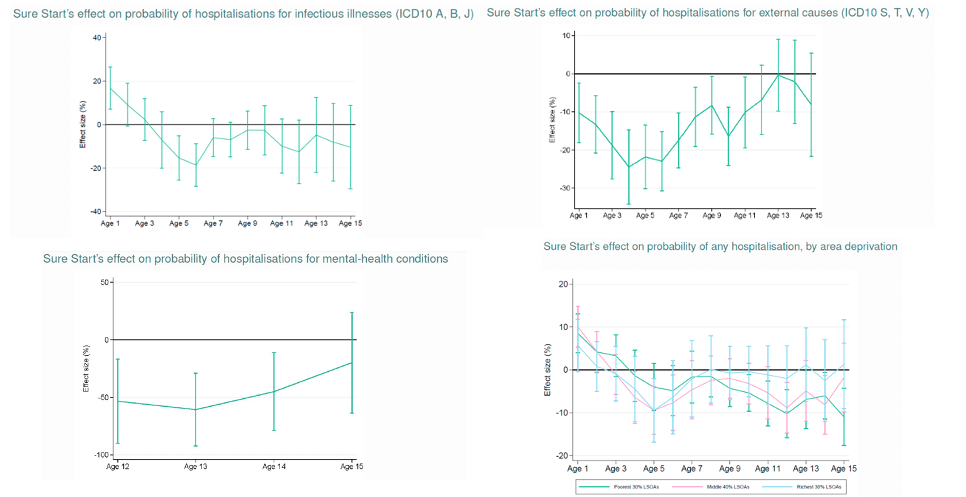
\includegraphics[width=13cm]{images/ch4/SS_bycauseandregion.png}
            \caption{Decomposition of the effect of Sure Start}
        \end{figure}
        \begin{itemize}        
            \item Greater access to Sure
            Start substantially increases hospitalisations for infectious illnesses in infancy, which can be because of referral effects or the spreading of the infectious disease in the childcare centres
            \item However, there are significant and substantial falls in hospitalisations because they build up a
            stronger immune response. This effect fade out in the longer term as the other kids' immune systems catch up after school
            \item Less hospitalisation due to external causes at early ages. Kids are able to fight with each other as they grow older
            \item Big reduction in hospitalisation for mental health at age of 12-13
            \item The program is more effective in poorer areas (poor = green; rich = light blue; middle = pink)
        \end{itemize}
    \end{itemize}

    
\section{Why do these programs work?}
This will help us understand the generalisability of programs implemented in one country at one time\\ \\
\textbf{How early interventions affect us later?}
\begin{itemize}
\item A stylised way
\begin{itemize}
    \item Health is a component of human capital, and good health will yield multiple returns later in life (e.g. education, earnings,...)
    \item Health can be developed throughout the lifecycle by human capital development (think about the factors involved in the production of health) and \textbf {\large{investments}} by parents and governments. Investments in human capital can be carried out at different stages in life.
    \item Investment level can also react to level of human capital
\end{itemize}
\item The shortfall with this very general approach is that there are so many ways to put money (can invest in pre-natal/ post-natal/ interventions at late childhood etc.). How to best allocate our money? 
\item Attanasio (2015) has developed a model that allows us to understand the impact of early childhood investments
\begin{itemize}
    \item This is a model of investment in children's human capital
    \item Parents are altruistic (care about child's human capital/ development), and they maximise utility function subject to constraints
    \item Human capital change over time because of (a) Investments, which can react to level of HK (b) Environmental variables whose evolution is independent of human capital (c) Past level of HK. Such process is governed by a production function
    \item This HK production function is complicated and non-linear
    \item The choice variable here is the level of parental investment to children, and parental behaviour plays an important role here - there can be compensation/reinforcement effects.
    \item Let's write this down formally. Here, I consider a simple framework where parents fully understand the child's human capital production function of:
    $$HK_{i,t+1}=g_t(HK_{i,t}, I_{i,t}, Z_{i,t}, e^{HK}_{i,t}) $$
\end{itemize}
Where
\begin{itemize}
    \item $HK_{i,t/t+1}$: Human capital
    \item $I_{i,t}$: Parental Investment
    \item $Z_{i,t}$: Other  background variables like parents' education
    \item $e^{HK}_{i,t}$ Random Shocks, or inputs in the production function that are not directly observed or considered by the researcher 
    \item Notice that the production function varies with time, and there is no saving
\end{itemize}

 \textbf{We then have the model in full glory}
\begin{maxi*}
    {C_{i,t},I_{i,t}}{U(C_{i,t}, HK_{i,t+1})}
    {}{}
    \addConstraint{C_{i,t}+P^I_t I_{i,t}=Y_{i,t}}\tag{Resource constraint}
    \addConstraint{HK_{i,t+1}= g_t(HK_{i,t}, I_{i,t}, Z_{i,t}, e^{HK}_{i,t})}\tag{Technological constraint}
\end{maxi*}
\begin{itemize}
    \item Here, $P^I_t$ is a vector of investment prices and the objective function is for parents
    \item Do not distinguish between material/time investment here
    \item Solving this model gives demand functions for investment and consumption
    \item Investment function is given by:
    $$I_{i,t}=f_t({HK_{i,t}; P^I_t; Z_{i,t}; e^{HK}_{i,t}; Y_{i,t}; \pi })$$
    Where $\pi$ is the vector of parameters characterising the utility and production function
    \item This is very important for empirical work, as this allows us to estimate the effect of early childhood investment on human capital (i.e. estimate the production function)
    \item More specifically, $P^I_t$ and $Y_{i,t}$ does not enter the production function, meaning that we can exploit variations in these variables to estimate the production function (Recall the way we estimate SEMs in ECON0019)
\end{itemize}
\end{itemize}
\section{Understanding the mechanisms}
We now have a good grasp of the reduced-form relationship between early childhood interventions and later life outcomes. But where does the better health of treated kids come from?
\begin{itemize}
    \item For example, in the Carolina Abecedarian Project, we see improved health when the treated kids turn 35. 
    \item Is it because of improvements in child development, or is it because of better education/ employment/ income of the treated kids later in life?
    \item \href{https://academic.oup.com/ej/article-abstract/126/596/F28/5077840?redirectedFrom=fulltext&casa_token=7tYaZ_u9hhsAAAAA:JtyABJ0NboRziZ1F73fmiYNF17TKsHa48wWG_hCynCAQ491LcMOp1GRP0DPh5HmN3DI1sWawzjkHA7k}{Conti et al. (2016)} showed that half of the impacts of the intervention are explained by early development (reduction in the child’s BMI and
increase in task orientation at ages 1-2)
            \begin{figure}[H]%option [H] means "strictly here"
    \centering
    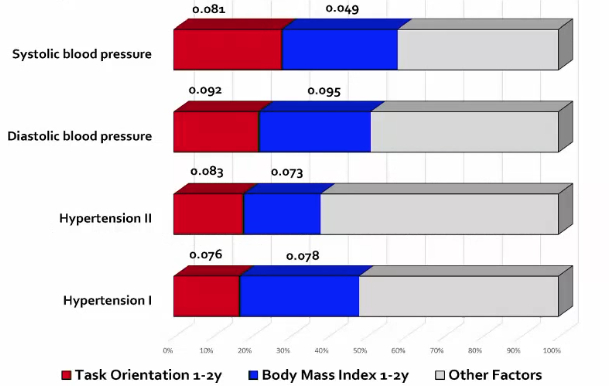
\includegraphics[width=13cm]{images/ch4/mechansms_ABC.png}
    \caption{Effectiveness of CAP explained by improvements in outcomes in early childhood}
    \end{figure}
\end{itemize}
    

